\documentclass[conference]{IEEEtran}

\usepackage{hyperref}
\usepackage{cite}
\usepackage{amsmath,amssymb,amsfonts}
\usepackage{algorithmic}
\usepackage{graphicx}
\usepackage{textcomp}
\usepackage{xcolor}
\usepackage{siunitx}
\def\BibTeX{{\rm B\kern-.05em{\sc i\kern-.025em b}\kern-.08em
    T\kern-.1667em\lower.7ex\hbox{E}\kern-.125emX}}
\begin{document}

\title{Exploring Cell counting with Neural Arithmetic Logic Units}

\author{\IEEEauthorblockN{Ashish Rana\IEEEauthorrefmark{1},
Taranveer Singh\IEEEauthorrefmark{2}, Harpreet Singh\IEEEauthorrefmark{3}, Neeraj Kumar\IEEEauthorrefmark{3} and Prashant Singh Rana\IEEEauthorrefmark{4}}
\IEEEauthorblockA{Department of Computer Science,
TIET Patiala, Punjab, India.\\
Email: \IEEEauthorrefmark{1}\{arana\_be15, tsingh\_me17, harpreet.s, neeraj.kumar, prashant.singh\}@thapar.edu
}}

\maketitle

\begin{abstract}

The big problem for neural network models which are trained to count instances is that whenever test range goes higher than training range generalization error increases i.e. they are not good generalizers outside training range. Consider the case of automating cell counting process where more dense images with higher cell counts are commonly encountered as compared to images used in training data. By making better predictions for higher ranges of cell count we are aiming to create better generalization systems for cell counting. With architecture proposal of neural arithmetic logic units (NALU) for arithmetic operations, task of counting has become feasible for higher numeric ranges which were not included in training data with better accuracy. As a part of our study we used these units and different other activation functions for learning cell counting task with two different architectures namely Fully Convolutional Regression Network and U-Net. These numerically biased units are added in the form of residual concatenated layers to original architectures and a comparative experimental study is done with these newly proposed changes . This comparative study is described in terms of optimizing regression loss problem from these models trained with extensive data augmentation techniques. We were able to achieve better results in our experiments of cell counting tasks with introduction of these numerically biased units to already existing architectures in the form of residual layer concatenation connections. Our experiments on a batch size of 16 shows a 20.22\% relative improvement as compared to original architecture and 34.84\% relative improvement on our custom created high count dataset created from BBBC005 synthetic cell count dataset achieving higher generalization capabilities for U-net based architectures. These results confirm that above mentioned numerically biased units does help models to learn numeric quantities for better generalization results.

\begin{IEEEkeywords}
Neural Arithmetic Logic Units, Cell Counting, ResNets, Fully Convolutional Regression Networks, U-net.
\end{IEEEkeywords}

\end{abstract}



\section{Introduction}

Ability to generalize concepts is fundamental component of intelligence and core for designing
smart systems \cite{b6, b7}. Neural networks simulates this behavior with hierarchical learning of concepts. When it comes to automation, counting is an important task from machine vision application \cite{b1} to cell counting \cite{b2}. While neural networks manipulates numerical quantities but it is not associated with systematic generalization \cite{b3, b4}. These networks fail to generalize as evident from high generalization error while predicting quantities that lie outside the training numerical range as shown in table \ref{tab:table1} or in figure \ref{fig5} elaborated in experiment section. This highlights memorization behavior in neural networks instead of generalization abilities.

Neural accumulators (NAC) and neural arithmetic logic units (NALU) \cite{b5} are biased to learn
systematic numerical computation and performs relatively better than non linear activation functions for arithmetic operations. This numerical bias of learning computations makes
them excellent choice for counting tasks which are essentially is an increment addition operation
only. Deep learning models generally take either segmentation approach with explicit counting trainer or end-to-end counting via a regression loss. In this paper we will go through the
latter approach \cite{b2} in detail for automation of cell counting process. As cell counting is cumbersome task and dense cell images with higher cell counts containing data outside training numeric range are common in real world scenarios. Achieving true cell automation with less generalization errors is the prime objective of this paper.

\begin{figure}[!h]
\centering
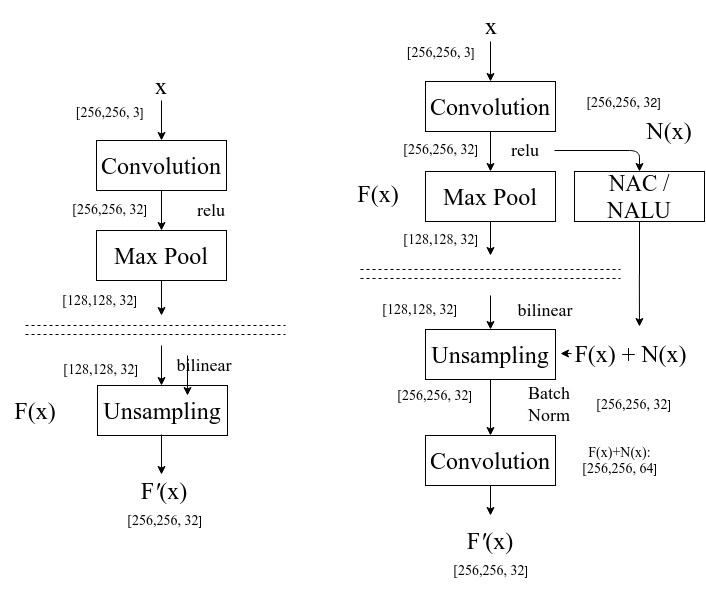
\includegraphics[width=0.45\textwidth]{assets/model-abstract-diagram.png}
\caption{Abstract representation of proposed modified architecture (\textit{Right}) with either neural accumulator (NAC) or neural arithmetic logic unit (NALU) as compared to previous Fully Convolution Regression Networks (\textit{Left}). Here, as clearly specified with dimensional analysis of tensor blocks (\textit{Right})  the layers in the newly proposed model are concatenated and again squeezed into same size as earlier  model architecture.}
\label{fig1}
\end{figure}

In regression loss approach Fully convolutional regression networks \cite{b2} and U-net \cite{b8} architectures learns mapping  between an image I(x) and a density map D(x), given by F$\colon$ I(x) $\rightarrow$ D(x) (I $\in$ R\textsuperscript{m $\times$ n} , D $\in$ R\textsuperscript{m $\times$ n} ) for a m $\times$ n pixel image. Later on, variations of these architectures with different activation functions are discussed in this paper. And their performance is compared with Neural accumulators (NAC) and Neural arithmetic logic units (NALU) concatenated architectures in the form of numerically biased residual connections , similar to ResNets \cite{b9} as shown in figure \ref{fig1} but instead of adding the previous layer input they are concatenated. On the surface, this proposed architecture changes leads to accuracy improvements due to increased model capacity with these numerically biased units. But, our results with custom high count dataset created from BBBC005 \cite{b29} reflects increased generalization counting abilities for high cell count images with higher relative decrease in mean absolute error(MAE).

Our concatenation based residual architecture utilizes the fundamentals of batch normalization like specified identity mapping architecture in ResNets \cite{b17}. But, instead of using convolution operation directly this network leverages numerical bias information obtained from NAC and NALU operations applied on input layer and then finally uses convolution operation on the concatenated layer. Before and after this concatenation of this numerical bias learning operation, batch normalization is carried out and output of this operation is added back again to our next main network layer, as shown in figure  \ref{fig1}.

With means of this paper we introduce changes in current regression based model architectures for end-to-end counter training and produce systems with higher accuracies for higher count testing ranges as well. Also, we validate our trained models on a different specially tailored validation dataset with approximately five times higher counts of cells as compared to training dataset created from BBBC005 synthetic cell dataset \cite{b29}.

\section{Related Work}

Intuitive numerical understanding is important in learning and by adjunct important in deep learning \cite{b6} for creating better models with higher generalization capabilities. Counting objects \cite{b10, b11, b12, b2, b14} in given image is a widely studied task. Trained models for counting tasks either use a deep learning model to segment instances of given object then count them in a post-processing step \cite{b15} or learn end-to-end predict count via a regression loss \cite{b2}. Networks like Count-ception \cite{b16} added the concept of average over redundant predictions with its deep Inception family network. Also, recent architectures like ResNets \cite{b17}, Highway Networks \cite{b18} and Densenets \cite{b19} advocate linear connections like Count-ception to promote better learning bias. Such models have better performance, though additional computational overhead due to increased depth of given architectures do arise. Our work highlights the generalization capabilities of the network, that extrapolate well on unseen parts of solution space which highlights underlying structure of behavior governing-equations \cite{b20}. We introduce architectural changes in models that learns residual functions and preserves input information which is numerically biased with reference to input layers. It is somewhat similar to ResNets \cite{b9}, which are easier to optimize and gain accuracy with increasing depth. With our experiments we aim to highlight that models with numerically biased concatenated residual functions helps in achieving better results with their addition in the form of a comparative study with original architectures. Also, with our results in this paper we demonstrate with our results that backpropagation learns this numerical bias without any explicit numeric quantity being provided as input implying that better computer vision counters can be trained with this module when added to existing convolutional neural network architectures.

Density based estimation doesn’t require prior object detection or segmentation \cite{b13, b21, b22}. In previous years, several works have investigated this approach. In \cite{b13}, the problem is stated as density estimation with a supervised learning algorithm, D(x) = c\textsuperscript{T}$\phi$(x), where D(x) represents  ground-truth density map, and $\phi$(x) represents  local features and parameters \textit{c} are learned by minimizing the error between predicted and true density with quadratic programming over all possible sub-windows. In \cite{b22}, regression forest is used to exploit patch-based idea for learning structured labels, then for new input image density map is estimated averaged over structured patch-based predictions. Also, in \cite{b21} an algorithm is used that allows fast interactive counting with ridge regression.

Cell counting \cite{b13} problem is classified into supervised learning problem that learns mapping between an image I(x) and a density map D(x), denoted by F$\colon$ I(x) $\rightarrow$ D(x) (I $\in$ R\textsuperscript{m $\times$ n} , D $\in$ R\textsuperscript{m $\times$ n} ) for a m $\times$ n pixel image, see figure \ref{fig2}. Density function D(x) function is defined on pixels in given image, integrating this map over an image region gives an estimate of number of cells in that region.  CNNs \cite{b23, b24} are quite popular in the bio-medical imaging because of their simple architecture and achieve great results. Like in mitosis detection \cite{b26}, neuronal membrane segmentation \cite{b25} and analysis of C. elegans embryos development \cite{b27}. Previously, fully convolutional regression networks (FCRNs) and Count-ception have given state-of-the-art results in cell counting, with potential for cell detection of overlapping cells.

\begin{figure}[!h]
\centering
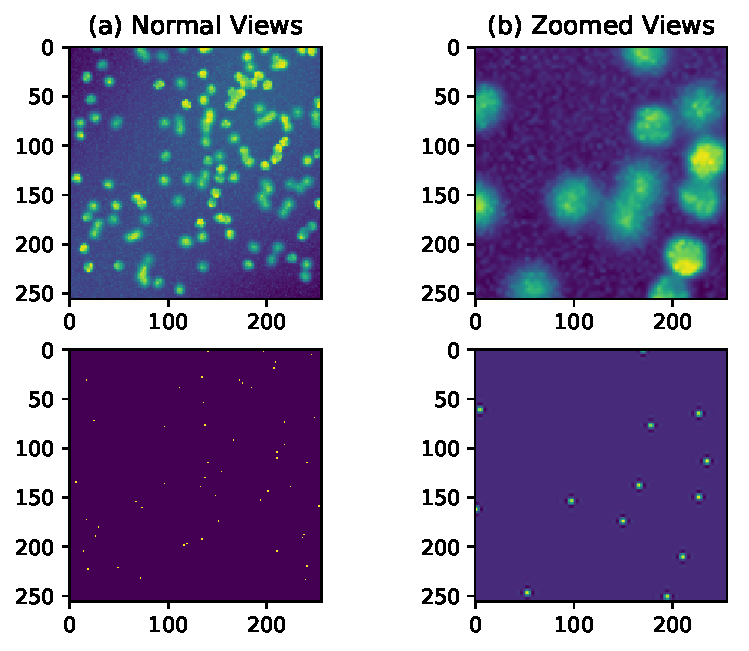
\includegraphics[width=0.45\textwidth]{assets/synthetic-cells-fig.pdf}
\caption{ \textbf{(a) Normal Views: } column represents training image in first row and corresponding annotated image in second row from synthetic dataset \cite{b28}. \textbf{(b) Zoomed Views: } This column represents zoomed in version of earlier mentioned images for better visualization.}
\label{fig2}
\end{figure}

Also, U-Nets \cite{b8} a type of fully convolutional network, uses a modified version of architecture proposed by Ciresan et al. \cite{b25} as latter is slow and trade-off between localization and use of context are present. In U-Nets pooling operations are replaced by upsampling operations to supplement usual contracting network. For localization high resolution features from contracting path are combined with unsampled output. Based on this information a successive convolution layer then learn to assemble more precise output. For our experimentation we selected fully convolution regression networks(FCRN) and U-net based on simple architecture and relative similarity in architecture with the difference being that U-net already uses inputs from previous layer for localization.

\section{Experiments}

In this section first we conceptually explore numerical accumulators (NACs) and numerical arithmetic logic units (NALUs) and compare their addition capabilities with multi-layer perceptrons equipped with different activation functions. With this study we aim to select concatenated residual connection variants from above mentioned numerically bias units which can best approximate the counting behavior and compare them with standard FCRN and U-net neural network architecture for regression loss approach in the following experiment done on synthetic dataset \cite{b28}. For validation of counting generalization achieved, our trained models are tested against synthetic cell image dataset with approximately five times higher counts than training data.

\subsection{Visual understanding of neural accumulators (NACs) and neural arithmetic logic units (NALUs)}

Neural accumulators (NACs) \cite{b5} supports accumulation of numerical quantities additively, a desirable bias for linear exploration while counting. It is special type of linear layer with transformation matrix \textbf{W} being continuous and differentiable parameterization for gradient descent. W = $\tanh$($\hat{W}$)$\odot$$\sigma$($\hat{M}$)  consists of elements in [-1, 1] with bias close to  −1, 0, and 1. See figure \ref{fig3} for ideation of this concept with following equations for NAC:  a = Wx, W = $\tanh$($\hat{W}$)$\odot$$\sigma$($\hat{M}$) where \textit{$\hat{W}$}, \textit{$\hat{M}$} are learning parameters and \textit{W} is transformation matrix.

\begin{figure}[!h]
\centering
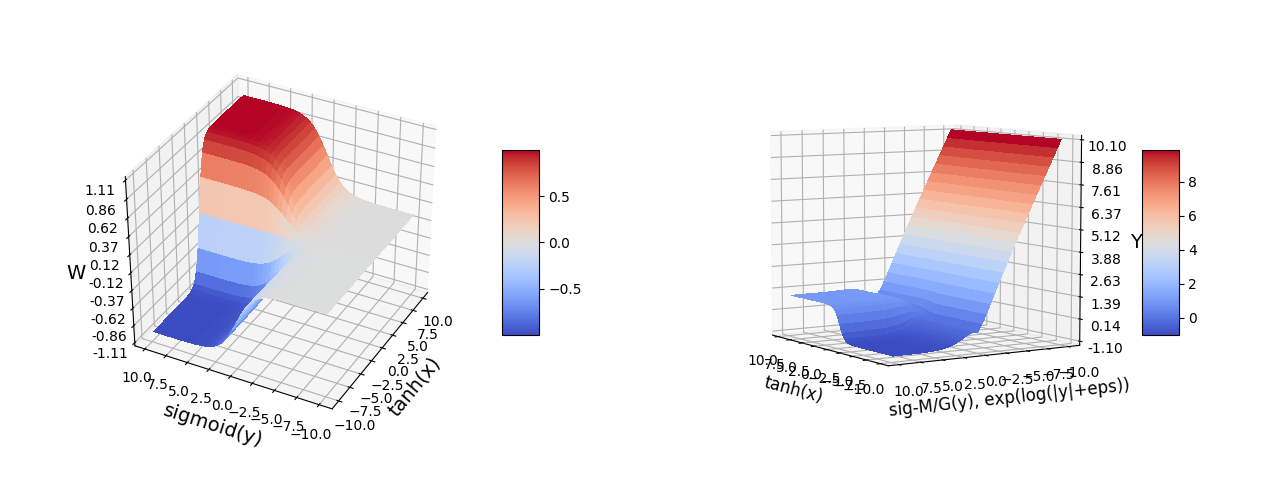
\includegraphics[width=0.45\textwidth]{assets/nac-nalu.png}
\caption{
\textbf{Left:} Neural accumulators (NACs) are biased towards learning [-1, 0, 1] as highlighted with large plateau regions around these values. This means its outputs are either addition or subtraction of input vectors not scaling.
\textbf{Right:} Approximate surface curve of neural arithmetic logic units (NALUs) with some dimensional constraints for 3-D plotting. It highlights the ability to scale, along with earlier numerical biases around [-1, 0, 1] as shown with plateau region surfaces.}
\label{fig3}
\end{figure}

For complex mathematical operations like multiplication and division we use neural arithmetic logic units (NALUs) \cite{b5}. It uses weighted sum of two sub-cells, one for addition or subtraction and another of multiply, division or power functions. It demonstrates that neural accumulators (NACs) can be extended for learning scaling operations with gate-controlled sub-operations. See figure \ref{fig3} for ideation of this concept with following equations for NALU: y = g$\odot$a + (1-g)$\odot$m; m = $\exp$W($\log$( $\mid$x$\mid$ + $\epsilon$)), g = $\sigma$(Gx) where \textit{m} is subcell that operates in \textit{log} space and \textit{g} is learned gate, both contains learning parameters.


\subsection{Comparative analysis of addition operation}

Here, we use neural networks with NACs/NALUs and multilayer perceptrons (MLP) with different activation functions but same structures. These are trained with two randomly generated inputs from uniform distribution \textit{a} and \textit{b} with each having 2\textsuperscript{14} data points for training. Prediction capabilities on test data with values ranging up to 10 times the training range are evaluated. Refer figure \ref{fig4} to observe architecture for both these trained models in this comparative experiment.

\begin{figure}[!h]
\centering
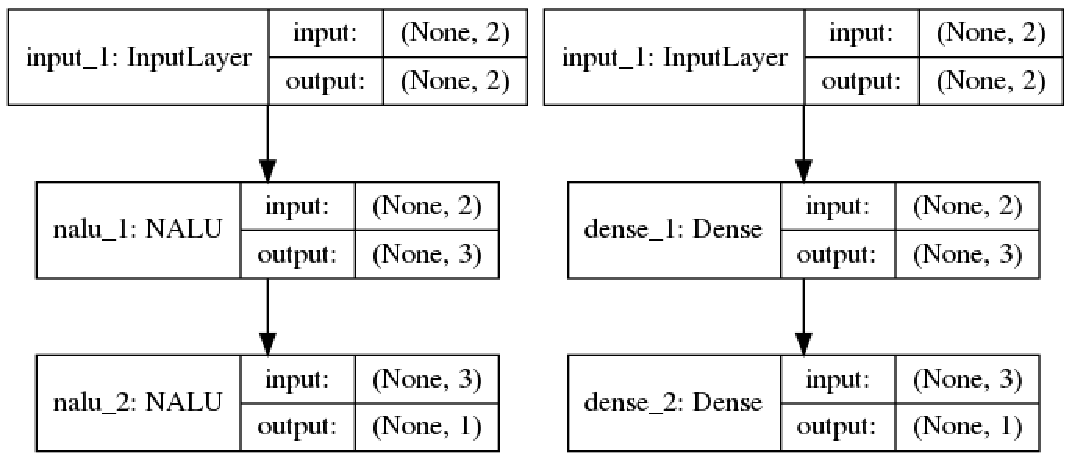
\includegraphics[width=0.45\textwidth]{assets/mlp-models.pdf}
\caption{The model on \textit{left} represents neural network with NAC or NALU units and on \textit{right} a multi-layer perceptron (MLP) which will be trained with different activation functions. Each variant of above models have two inputs, three hidden units, one output.}
\label{fig4}
\end{figure}

Comparative analysis is summarized in table  \ref{tab:table1} with mean absolute error (MAE) as an accuracy measure for MLP variants, NAC, NALU and its variants with changed learned gate for extrapolation. Also, in NALU-Tanh and NALU-Hard Sigmoid the learning gate \textit{g's} is changed to observe any improvements in NALU's performance based on this change.


\bgroup
\def\arraystretch{1.25}
\begin{table}[h!]
  \begin{center}
    \caption{\textbf{Comparative result summarization for multiple models}}
    \label{tab:table1}
    \begin{tabular}{|c|c|}
    
    \hline
      \textbf{Layer Configuration/Activations} & \textbf{Mean Absolute Error (\textit{a+b})} \\
    \hline

     Linear MLP & \num{3.63e-06}\\
     \hline
     Sigmoid MLP & \num{29.830}\\
     \hline
     Tanh MLP & \num{15.743}\\
     \hline
     ELu MLP & \num{0.019}\\
     \hline
     ReLU MLP & \num{0.001}\\
     \hline
     Leaky ReLU MLP & \num{9.83e-04}\\
     \hline
     PReLU MLP & \num{0.001}\\
     \hline
     NAC & \num{2.70e-06}\\
     \hline
     NALU & \num{2.71e-06}\\
     \hline
     NALU-Hard Sigmoid & \num{3.24e-06}\\
     \hline
     NALU-Tanh & \num{3.18e-06}\\
     \hline
    \end{tabular}
  \end{center}
\end{table}
\egroup

From these results stated in table \ref{tab:table1} and visualized in figure \ref{fig5} we conclude that Linear, LeakyReLU, ReLU activations and NAC, NALU, NALU-Tanh modules were the top performers in extrapolation task for numeric addition operation task. Hence, these top performers are used further in cell-counting task on synthetic dataset for learning end-to-end counting mechanism.

\begin{figure}[!h]
\centering
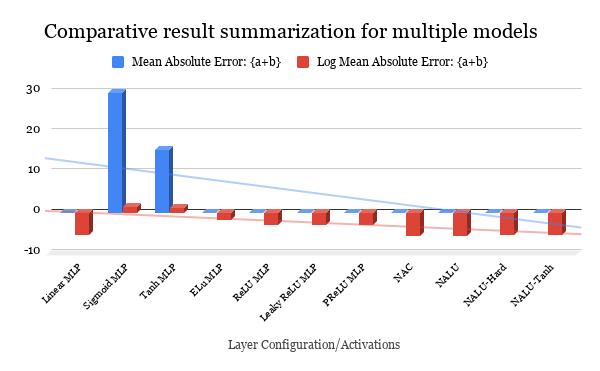
\includegraphics[width=0.45\textwidth]{assets/comparative-model-results.png}
\caption{Above visualization of Mean Absolute Error and log\textsubscript{10}(Mean Absolute Error) for different models learning identity mapping, demonstrates that our standard activation functions like \textit{sigmoid} and \textit{tanh} doesn't perform that well with higher data ranges during testing. Whereas, \textit{NACs} and \textit{NALUs} clearly overpowers the identity learning task and \textit{linear}, \textit{relu} based activation functions somewhat manages to provide sane results.}
\label{fig5}
\end{figure}


\subsection{Counting experiment}

\footnote{\textit{Code repository:} \url{https://github.com/ashishrana160796/nalu-cell-counting}}

In this experiment section the first subsections elaborates the datasets used for training and validation of our trained models, plus the data augmentation techniques used in our experiment. After that we elaborate onto different architectures used for training having different activation layers on standard architectures and residual concatenated connection modules on modified proposed model architectures.

\subsubsection{Datasets and data augmentation}

Synthetic dataset which is generated by system \cite{b28}. 200 highly-realistic synthetic fluorescence microscopic images of bacterial cells are used for experimentation with a 75/25 train-test split for training each model architecture and its variants. Images are having average of 174±64 cells.

For validation of trained models and checking true generalization capabilities we use BBBC005 from the the Broad Institute’s Bioimage Benchmark Collection \cite{b29}. 600 images have a corresponding foreground mask are classified as completely in-focus for ground truth. We take a subset of this dataset with highly focused \textit{F1} images only and coalesce image into one after replicate same image 16 times with some padding around each sub-image. After these changes the ground truth values are accordingly changed and then image is resized to the same dimensions as original dataset, see figure \ref{fig6}.

\begin{figure}[!h]
\centering
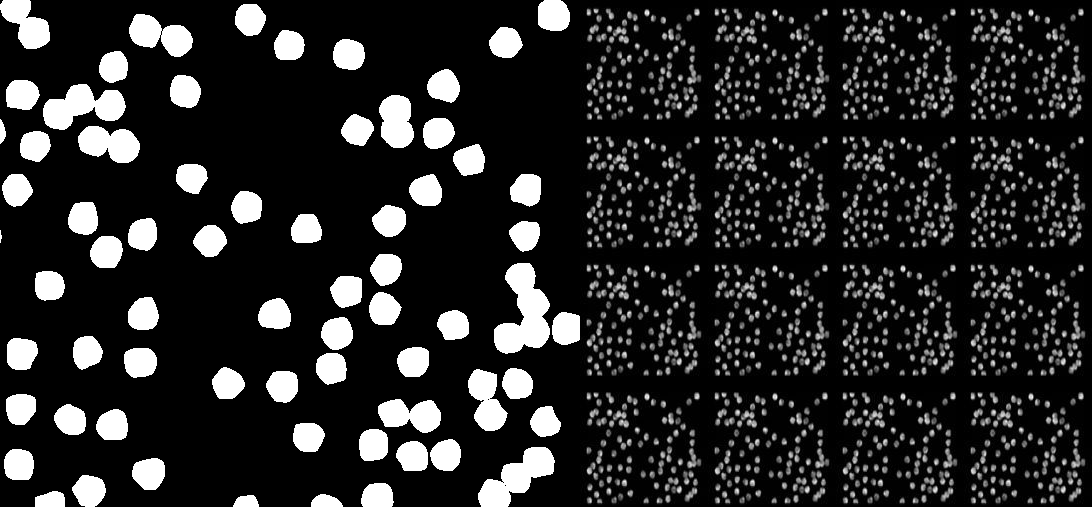
\includegraphics[width=0.45\textwidth]{assets/bbbc005-custom-dataset.png}
\caption{\textit{Left: }Original image from BBBC005 dataset. \textit{Right: }Repeated image generated from a \textit{4X4} grid repetition operation.}
\label{fig6}
\end{figure}

Data augmentation with elastic deformations to training images is applied for teaching network the desired invariance and robustness properties, like specified in figure \ref{fig8}. These elastic deformations are introduced in the form of angular shear in the training images. Translation and rotation invariance along with robustness to gray value variations and deformations is main focus of augmentation process for microscopic images. Disfigurement using random displacement vectors on a coarse 3x3 grid were also generated. These data augmentation techniques especially are helpful for our custom data which is created just by repeating the original image in order to supplement a more robust dataset for the model to train on.

\begin{figure}[!h]
\centering
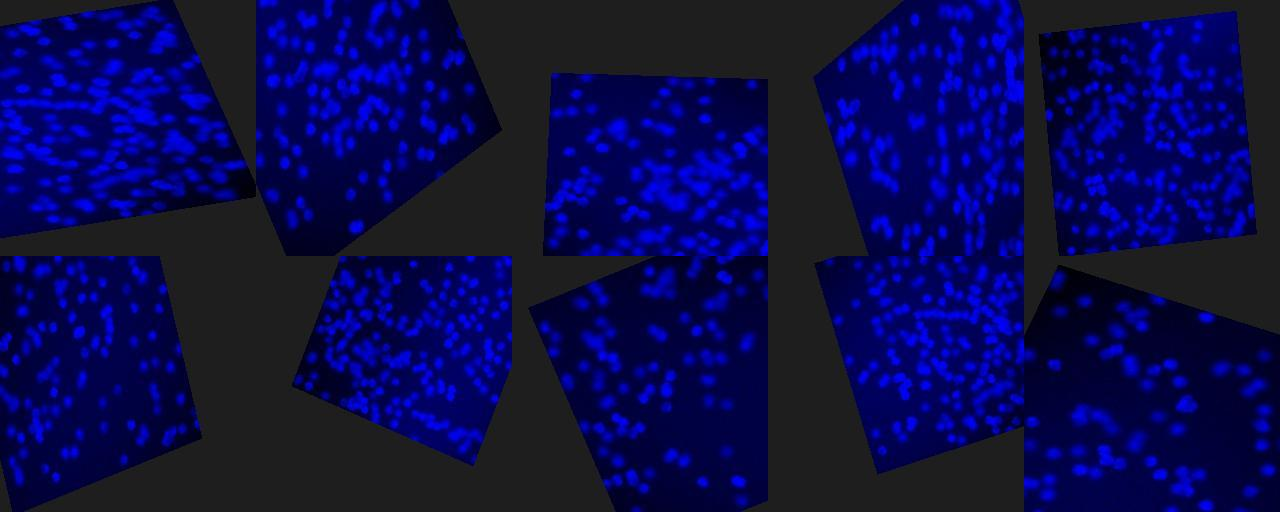
\includegraphics[width=0.45\textwidth]{assets/data-aug.png}
\caption{This figure specifies ten different types of elastic deformations for the input images and corresponding target images are also deformed in such manner for more robust training. }
\label{fig7}
\end{figure}

\subsubsection{Defining regression task and architecture details}

In training dataset ground truth is provided as dot annotation corresponding to each cell. For training, dot annotations are represented by Gaussian and density surface D(x) which is formed from superposition of Gaussians. The optimization task is to regress density surface from corresponding image I(x). This is achieved by training convolutional neural networks (CNN) using mean square error between output heat map and target density surface as the loss function. Hence, at inference given an input I(x), the model predicts density heat map D(x).

FCRNs are inspired from VGG-net, we only used small kernels of size 3x3 pixels. Feature maps are increased for avoiding spatial information loss. Activation layers like convolution-ReLU-Pooling are popular in CNN architectures \cite{b23}. Here, we have altered these layers to create different activation maps which contains some numerical bias in the form of residual connections and regularization by batch normalization. The first layers contains convolutions-pooling operations, then we undo spatial reduction by upsampling operations for learning end-to-end training. Also, for dimensional compatibility of residual NAC or NALU modules we did pooling and upsampling operations on these residual modules after batch normalization. See figure \ref{fig8} for comparison between earlier original model and newly proposed architecture along with parameter details.

\begin{figure}[!h]
\centering
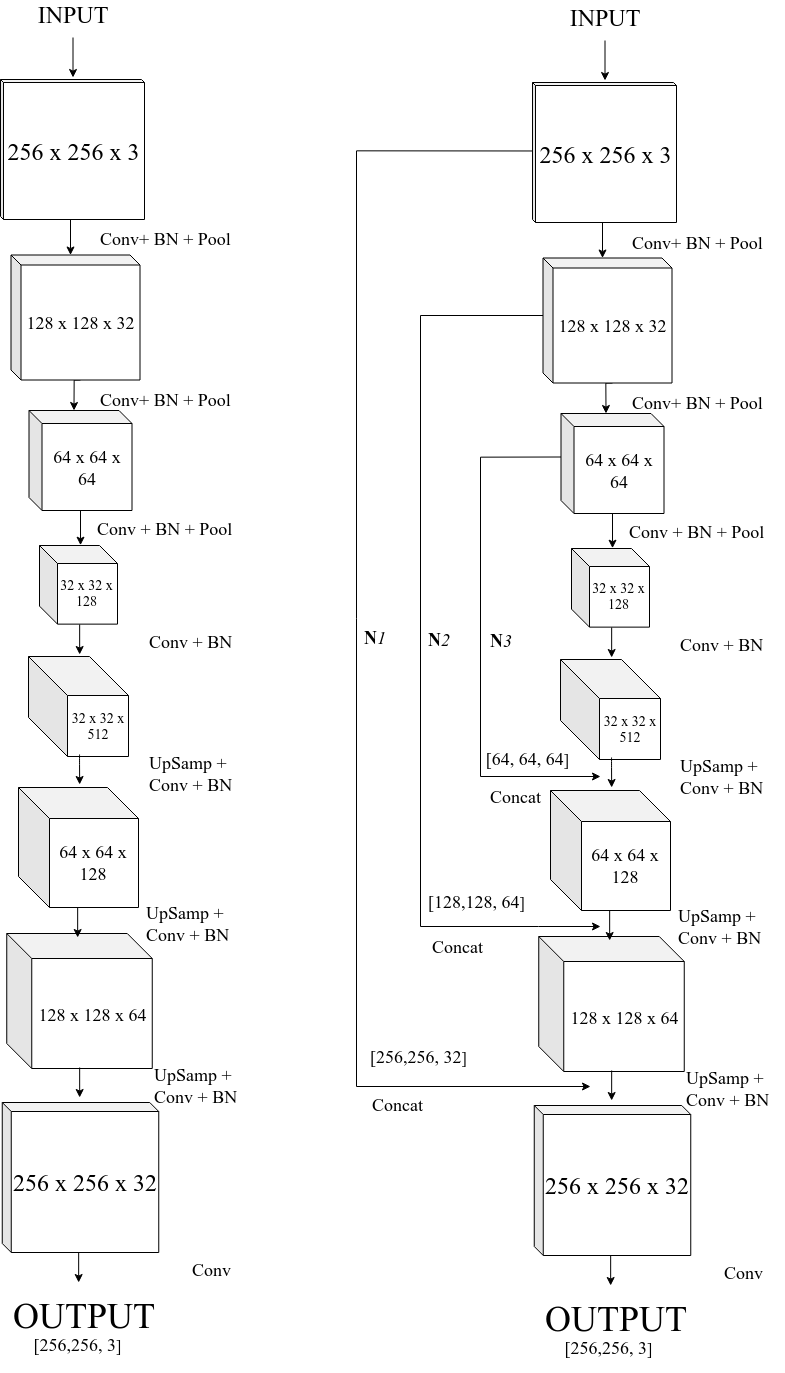
\includegraphics[width=0.35\textwidth]{assets/fcrn-nalu.png}
\caption{\textit{Network Structure Left: }FCRN with 3x3 convolution operations. \textit{Network Structure Right: } FCRN added with residual concatenation connections of \textbf{N}\textit{i} numerically biases units. Also, for dimensional compatibility \textbf{N}\textit{i} residual layers are fed to corresponding main network layers and after that normalized for regularization. At last, 1x1 \textbf{Conv} operation output in the form of density map of result image is generated .\newline
\textbf{Conv + BN + Pool: }A 3x3 convolutional operation with batch normalization regularization and  2x2 max pooling layer.\newline
\textbf{Unsample+Conv + BN: }Unsampling + Convolutional operation with batch normalization regularization.\newline
\textbf{Concat: }Feature maps concatenated along depth dimension.\newline
\textbf{N\textit{i}: }NAC or Variants of NALUs as residual concatenated connection.
}
\label{fig8}
\end{figure}

U-net is modified upon the previously discussed FCRN architecture by having large number of feature channels for upsampling to propagate context information to high resolution layers. That makes expansive path almost symmetric to contracting path yielding a u-shape. Similar to above FCRNs optimization problem formulation remains the same, residual concatenated connection addition with NACs and NALU units along with batch normalization is done. Also, U-net architecture used in this paper is more computationally expensive than FCRN having approximately thrice the number of parameters leading to more feature learning capacity. See figure \ref{fig9} for comparison between earlier original U-net model and newly proposed architecture along with parameter details.

\begin{figure}[!h]
\centering
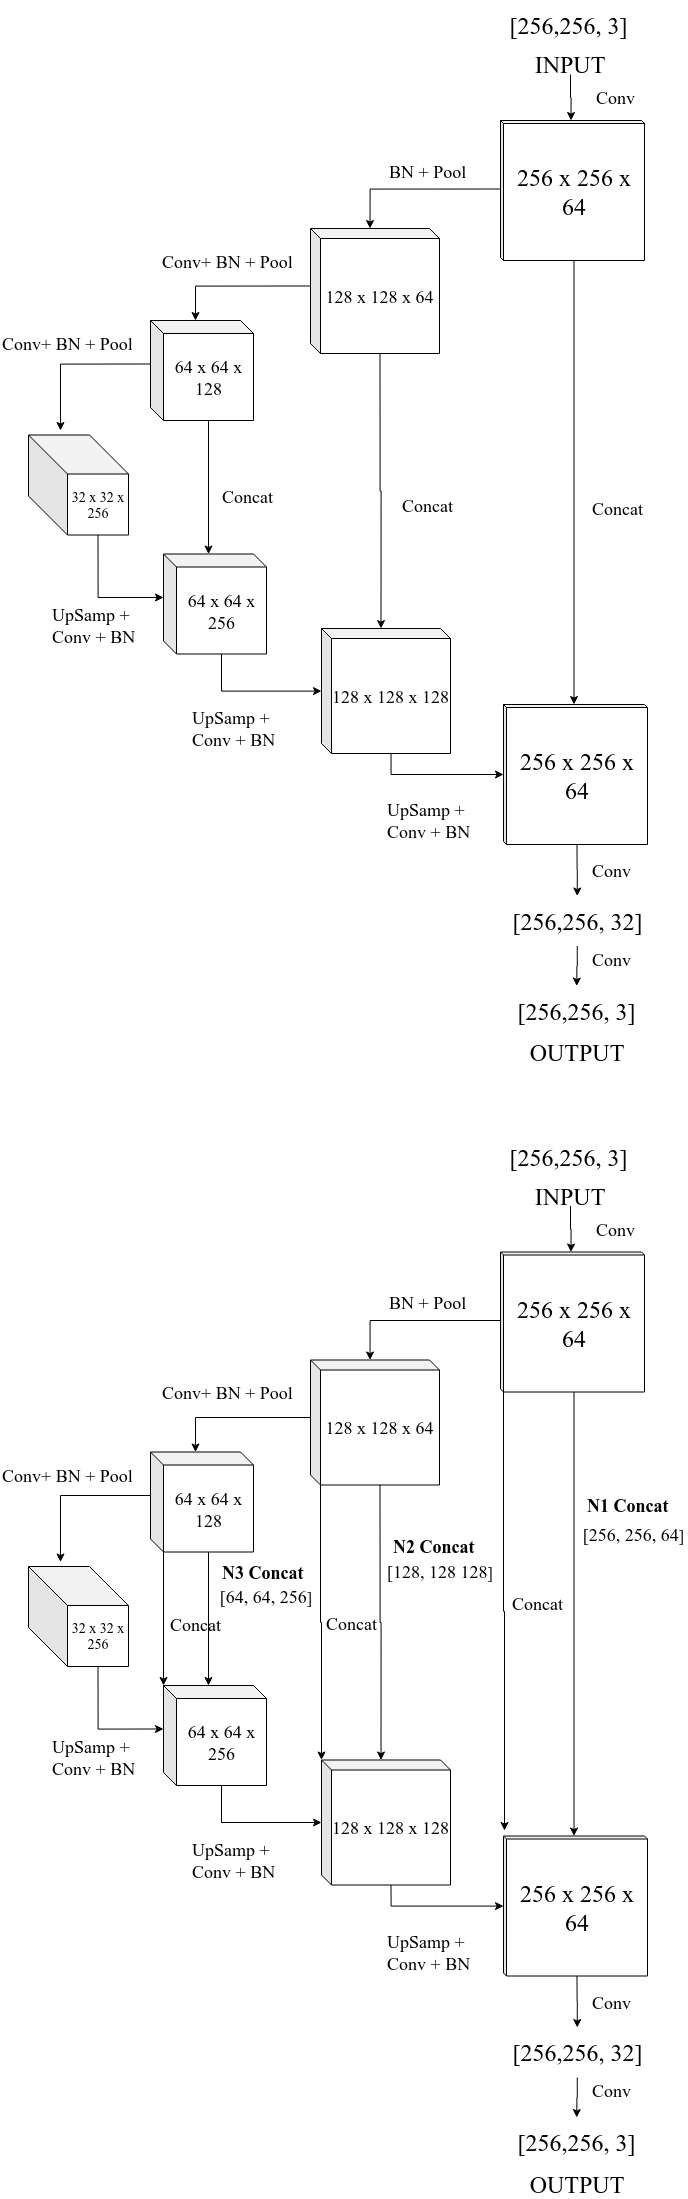
\includegraphics[width=0.30\textwidth]{assets/u-net-nalu.png}
\caption{\textit{Network Structure Top: }U-net with 3x3 convolution operations and increasing depth of filters from 64 to 256 for feature abstraction \& learning and after that these layers are fed to upsampling layers. \textit{Network Structure Bottom: } U-nets added with residual concatenation connections of \textbf{N}\textit{i} numerically biased units and after concatenation they are batch normalization for regularization. Finally, the last 1x1 \textbf{Conv} operation output in the form of density map is generated. Operations annotations are same as mentioned in figure \ref{fig8} \newline}
\label{fig9}
\end{figure}

For the concatenation of residual connections of these units the dimensional consistency is maintained by added pooling and upsampling operations accordingly for these units to merge with the base network. FCRN’s implementation resembles that of MatConvNet \cite{b30} as upsampling in Keras is implemented by repeating elements, instead of bilinear sampling. In U-nets \cite{b8}, for implementation low-level feature representations are fused during upsampling, aiming to compensate the information loss due to max pooling.

\section{Results}

Mean absolute error (MAE) is the metric used in this paper for measuring results for cell counting on the synthetic cell dataset \cite{b28} and custom BBBC005 synthetic modified high cell count validation dataset.

\begin{itemize}
\item \textbf{Mean Absolute Error (MAE):}
Mean Absolute Error (MAE): The mean absolute error is an average of the difference between the predicted value and true value.
\begin{equation}
AE = \|e_i\| = \|y_i - x_i\|
\end{equation}
\begin{equation}
MAE = \sum_{i=1}^{n} \frac{|e_i|}{n}
\end{equation}
\end{itemize}

\begin{itemize}
\item \textbf{Relative Improvement  Percentage}
Relative Improvement  Percentage (RIP): Here, in context of this paper it defined as percentage improvement in MAE of a given model with respect to baseline ReLU models for FCRN and U-net architectures. In below equation, M\textsubscript{r} is MAE from baseline ReLU model and M\textsubscript{i} is model under consideration.
\begin{equation}
 RIP_\% = ((M_r - M_i) / M_r) * 100
\end{equation}

\end{itemize}




Result table \ref{tab:table2} compares earlier FCRN, U-net architectures with new numerically biased ResNet like  connection modules with NACs and NALUs units under current training setup. With our setup we able to obtain similar results as mentioned in earlier reference papers and also we have equipped earlier model architectures with different regularization activations as specified in the table. From earlier ReLU implementation clearly Linear and LeakyReLU activation regularization based models have performed well. Also, for both model structures NAC and NALUs residual modules have outperformed all the earlier specified regular FCRN architecture. And similar arguments and results are extended by U-net model results where NALU layer concatenation based U-net outperforms all the models trained for our experiment.

\bgroup
\def\arraystretch{1.25}
\begin{table}[h!]
  \begin{center}
    \caption{\textbf{Result summarization for trained models}}
    \label{tab:table2}
    \begin{tabular}{|c|c|c|c|}
    
    \hline
      \textbf{FCRN-Models} & \textbf{MAE} & \textbf{U-Net-Models} & \textbf{MAE} \\
    \hline

     ReLU  & 3.43 & ReLU & 1.78\\
     LeakyReLU  & 3.39 & LeakyReLU & 1.74\\
     Linear  & 3.34 & Linear & 1.73\\
	 NALU-tanh & 3.21 & NALU/tanh & 1.56\\
	 NALU & \textbf{3.17} & NALU & \textbf{1.42}\\
     NAC & 3.23 & NAC & 1.63\\
     
     \hline
     \end{tabular}
  \end{center}
\end{table}
\egroup


Result table \ref{tab:table3} compares performance of above trained models on a new validation dataset containing much higher cell counts for measuring performance on extrapolation capabilities counting tasks. For validation set we have used 300 images of size 256x256 pixels with cell counts averaging around 1200±12. Here also, NAC and NALU based residual concatenation module based models outperforms earlier architectures for counting tasks. This time relative improvement in even more for FCRN and U-net models showcasing better generalization abilities of trained models.

\bgroup
\def\arraystretch{1.25}
\begin{table}[h!]
  \begin{center}
    \caption{\textbf{Validating trained models for extrapolation cell counting tasks}}
    \label{tab:table3}
    \begin{tabular}{|c|c|c|c|}
     
         \hline
      \textbf{FCRN-Models} & \textbf{MAE} & \textbf{U-Net-Models} & \textbf{MAE} \\
    \hline

     ReLU  & 3.04 & ReLU & 2.87\\
     LeakyReLU  & 2.99 & LeakyReLU & 2.62\\
     Linear  & 2.85 & Linear & 2.47\\
	 NALU-tanh & 2.32 & NALU-tanh & 1.95\\
	 NALU & \textbf{2.27} & NALU & \textbf{1.87}\\
     NAC & 2.40 & NAC & 1.92\\
    
     \hline
     \end{tabular}
  \end{center}
\end{table}
\egroup

Relative improvement in predictions is visualized in figure \ref{fig10} against ReLU based regularization as base result for comparison with other regularization layer based changes in FCRNs \& U-nets and concatenation layer NALU/NAC residual connection addition in FCRNs \& U-nets. It includes averaged out comparison from multiple executions of training and testing runs for both interpolation testing and extrapolation validation counting tasks for FCRN and U-net variant models with respect to ReLU based FCRN and U-net model. From, this figure it is clearly highlighted that models with NAC and NALUs residual modules have better generalization capabilities for extrapolation counting tasks i.e. they are better generalizers for this given cell counting task with increase in relative improvement in prediction as compared to base ReLU implementation. This figure shows more increase in relative improvement as we move right towards horizontal axis for both testing and validation task with extrapolation where in validation extrapolation task NAC/NALU models performing even better than testing data from which we can conclude that trained models are having better generalization abilities with some learned numerical bias in their trained weights with which even better predictions for higher count cells is made.



\begin{figure}[!h]
\centering
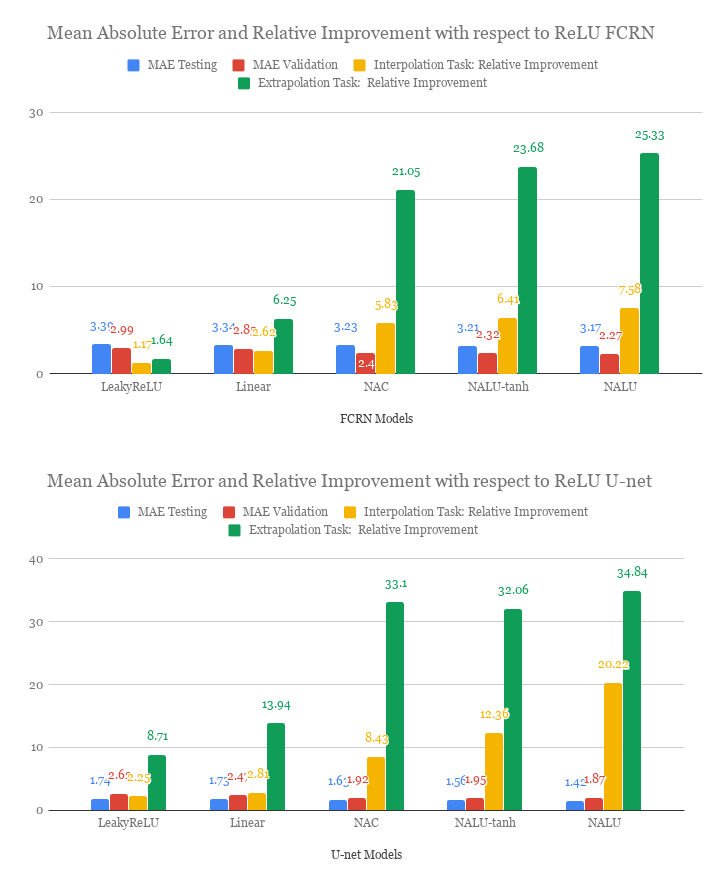
\includegraphics[width=0.50\textwidth]{assets/merged-relative-improv-results.png}
\caption{Moving towards right in above figure and measuring percentage relative improvement metric there is sharp increase with NALU and NAC units based models highlighting increase in relative improvement with respect to baseline ReLU models is even more for extrapolation tasks. For interpolation task there is highest 9\% improvement and for extrapolation there is 23\% improvement with NAC units as residual connection.}
\label{fig10}
\end{figure}

\section{Summary}
We were able to show that addition of newly proposed NACs and NALU units in existing architectures in the form of residual concatenation connection layer modules achieves better results. With numerically biased residual connections, higher accuracy for more dense images having higher counts of cells is achieved. Hence, producing more generalized cell counters that provides better predictions for real life use-cases. Finally, for code implementation details and other extra experimental results refer to this paper's  \href{https://github.com/ashishrana160796/nalu-cell-counting}{github repository}.

\begin{thebibliography}{00}
\bibitem{b1} Baygin, Mehmet, et al. "An Image Processing based Object Counting Approach for Machine Vision Application." arXiv preprint arXiv:1802.05911 (2018).
\bibitem{b2} Xie, Weidi, J. Alison Noble, and Andrew Zisserman. "Microscopy cell counting and detection with fully convolutional regression networks." Computer methods in biomechanics and biomedical engineering: Imaging \& Visualization 6.3 (2018): 283-292.
\bibitem{b3}Fodor, Jerry A., and Zenon W. Pylyshyn. "Connectionism and cognitive architecture: A critical analysis." Cognition 28.1-2 (1988): 3-71.
\bibitem{b4}Marcus, Gary F. The algebraic mind: Integrating connectionism and cognitive science. MIT press, 2018.
\bibitem{b5} Trask, Andrew, et al. "Neural arithmetic logic units." Advances in Neural Information Processing Systems. 2018.
\bibitem{b6}  Dehaene, Stanislas. The number sense: How the mind creates mathematics. OUP USA, 2011.
\bibitem{b7} Gallistel, C. Randy. "Finding numbers in the brain." Philosophical Transactions of the Royal Society B: Biological Sciences 373.1740 (2018): 20170119.
\bibitem{b8} Ronneberger, Olaf, Philipp Fischer, and Thomas Brox. "U-net: Convolutional networks for biomedical image segmentation." International Conference on Medical image computing and computer-assisted intervention. Springer, Cham, 2015.
\bibitem{b9} He, Kaiming, et al. "Deep residual learning for image recognition." Proceedings of the IEEE conference on computer vision and pattern recognition. 2016.
\bibitem{b10} Arteta, Carlos, et al. "Interactive object counting." European conference on computer vision. Springer, Cham, 2014.
\bibitem{b11} Chan, Antoni B., Zhang-Sheng John Liang, and Nuno Vasconcelos. "Privacy preserving crowd monitoring: Counting people without people models or tracking." 2008 IEEE Conference on Computer Vision and Pattern Recognition. IEEE, 2008.
\bibitem{b12}Seguí, Santi, Oriol Pujol, and Jordi Vitria. "Learning to count with deep object features." Proceedings of the IEEE Conference on Computer Vision and Pattern Recognition Workshops. 2015.
\bibitem{b13} Lempitsky, Victor, and Andrew Zisserman. "Learning to count objects in images." Advances in neural information processing systems. 2010.
\bibitem{b14} Zhang, Cong, et al. "Cross-scene crowd counting via deep convolutional neural networks." Proceedings of the IEEE conference on computer vision and pattern recognition. 2015.
\bibitem{b15} Hernández, Carlos X., Mohammad M. Sultan, and Vijay S. Pande. "Using Deep Learning for Segmentation and Counting within Microscopy Data." arXiv preprint arXiv:1802.10548 (2018).
\bibitem{b16} Paul Cohen, Joseph, et al. "Count-ception: Counting by fully convolutional redundant counting." Proceedings of the IEEE International Conference on Computer Vision. 2017.
\bibitem{b17} He, Kaiming, et al. "Identity mappings in deep residual networks." European conference on computer vision. Springer, Cham, 2016.
\bibitem{b18} Srivastava, Rupesh Kumar, Klaus Greff, and Jürgen Schmidhuber. "Highway networks." arXiv preprint arXiv:1505.00387 (2015).
\bibitem{b19} Huang, Gao, et al. "Densely connected convolutional networks." Proceedings of the IEEE conference on computer vision and pattern recognition. 2017.
\bibitem{b20} Brunton, Steven L., Joshua L. Proctor, and J. Nathan Kutz. "Discovering governing equations from data by sparse identification of nonlinear dynamical systems." Proceedings of the National Academy of Sciences 113.15 (2016): 3932-3937.
\bibitem{b21} Arteta, Carlos, et al. "Interactive object counting." European conference on computer vision. Springer, Cham, 2014.
\bibitem{b22} Fiaschi, Luca, et al. "Learning to count with regression forest and structured labels." Proceedings of the 21st International Conference on Pattern Recognition (ICPR2012). IEEE, 2012.
\bibitem{b23}Krizhevsky, Alex, Ilya Sutskever, and Geoffrey E. Hinton. "Imagenet classification with deep convolutional neural networks." Advances in neural information processing systems. 2012.
\bibitem{b24} LeCun, Yann, et al. "Gradient-based learning applied to document recognition." Proceedings of the IEEE 86.11 (1998): 2278-2324.
\bibitem{b25} Ciresan, Dan, et al. "Deep neural networks segment neuronal membranes in electron microscopy images." Advances in neural information processing systems. 2012.
\bibitem{b26} Cireşan, Dan C., et al. "Mitosis detection in breast cancer histology images with deep neural networks." International Conference on Medical Image Computing and Computer-assisted Intervention. Springer, Berlin, Heidelberg, 2013.
\bibitem{b27}Ning, Feng, et al. "Toward automatic phenotyping of developing embryos from videos." IEEE Transactions on Image Processing 14 (2005): 1360-1371.
\bibitem{b28} Lehmussola, Antti, et al. "Computational framework for simulating fluorescence microscope images with cell populations." IEEE transactions on medical imaging 26.7 (2007): 1010-1016.
\bibitem{b29}Ljosa, Vebjorn, Katherine L. Sokolnicki, and Anne E. Carpenter. "Annotated high-throughput microscopy image sets for validation." Nature methods 9.7 (2012): 637-637.
\bibitem{b30} Vedaldi, Andrea, and Karel Lenc. "Matconvnet: Convolutional neural networks for matlab." Proceedings of the 23rd ACM international conference on Multimedia. ACM, 2015.
\end{thebibliography}
\end{document}